\documentclass[10pt,a4paper]{article}
\usepackage[utf8]{inputenc}
\usepackage[T1]{fontenc}
\usepackage{amsmath}
\usepackage{amsthm}
\usepackage{amssymb}
\usepackage{graphicx}
\usepackage{mathtools}
\usepackage[ruled,vlined,linesnumbered]{algorithm2e}
\usepackage[left=2.50cm, right=2.50cm, top=2.0cm, bottom=2.0cm]{geometry}


\makeatother
\DeclareMathOperator*{\argmin}{argmin}
\DeclareMathOperator*{\Max}{\text{max}}
\DeclareMathOperator*{\E}{\mathbb{E}}
\newcommand{\Ei}[1]{\mathbb{E}_{#1}}
\DeclareMathOperator*{\Eik}{\mathbb{E}_{\mathit{i_k}}}
\DeclareMathOperator*{\Eikplus}{\mathbb{E}_{\mathit{i_{k+1}}}}
\newcommand{\Eiplus}[1]{\mathbb{E}_{i_{#1}}}
\DeclareMathOperator*{\LC}{\text{\textup{LC}}^1}
\DeclareMathOperator*{\grad}{\mathit{\nabla \!f}}
\DeclareMathOperator*{\argmax}{arg\;max}
\DeclareMathOperator*{\gradik}{\mathit{\nabla\!\fik}}
\DeclareMathOperator*{\Lmax}{\mathit{L_{max}}}
\newcommand{\R}{\mathbb{R}}
\newcommand{\st}{\text{s.t.} \;\;\;}
\newcommand{\Rn}{\mathbb{R}^n}
\newcommand{\ikplus}{i_{k+1}}
\newcommand{\wrefi}[2]{w_{r(#1, i_{#2})}}
\newcommand{\wref}[1]{\wrefi{#1}{#1}}
\newcommand{\fik}{f_{i_k}}
\newcommand{\fikofwstar}{\fik(w^*)}
\newcommand{\fofwstar}{f(w^*)}
\newcommand{\fii}[1]{f_{i_{#1}}}
\newcommand{\fikplus}{f_{i_{k+1}}}
\newcommand{\fiplus}[1]{f_{i_{#1}}}
\newcommand{\fimax}{f_i^{\text{max}}}
\newcommand{\fikmax}{\fik^{\text{max}}}
\newcommand{\bmax}{b_{\text{max}}}
\newcommand{\fmax}{f^{\text{max}}}
\newcommand{\fmaxk}[1]{f_{i_{#1}}^{\text{max}}}
\newcommand{\Lik}{L_{i_k}}
\newcommand{\Cik}{C_{i_k}}
\newcommand{\deltak}{\delta^{l_k}}
\newcommand{\deltakplus}{\delta^{l_k+1}}
\newcommand{\deltakminus}{\delta^{l_k-1}}
\newcommand{\etatilde}{\tilde{\eta}_{k,0}}
\newcommand{\muik}{\mu_{i_k}}
\newcommand{\etamax}{\eta^{\text{max}}}
\newcommand{\etamaxx}{\bar{\eta}^{\text{max}}}
\newcommand{\etamin}{\eta^{\text{min}}}
\newcommand{\etaminn}{\bar{\eta}^{\text{min}}}
\newcommand{\minimum}[2]{\min \left\{ #1, #2 \right \} }
\newcommand{\maximum}[2]{\max \left\{ #1, #2 \right \} }
\newcommand{\W}[1]{{\scriptscriptstyle W #1}}
\newcommand{\gradi}[1]{\nabla f_{i_{#1}} (w_{i_{#1}}) }
\makeatletter

\newtheorem{assumption}{Assumption}
\newtheorem{lemma}{Lemma}
\newtheorem{proposition}{Proposition}
\newtheorem{theorem}{Theorem}
\newtheorem{corollary}{Corollary}
\newtheorem{remark}{Remark}


\newcommand{\imgS}{.26}
\newcommand{\dir}{exp1/}
\newcommand{\model}{mlp}
\newcommand{\modelname}{mlp}


\newcommand{\mlp}{{\texttt{mnist|mlp}}}
\newcommand{\res}{{\texttt{cifar10|resnet34}}}
\newcommand{\dense}{{\texttt{cifar10|densenet121}}}
\newcommand{\ress}{{\texttt{cifar100|resnet34}}}
\newcommand{\denses}{{\texttt{cifar100|densenet121}}}
\newcommand{\fashion}{{\texttt{fashion|effb1}}}
\newcommand{\svhn}{{\texttt{svhn|wrn}}}
\newcommand{\wiki}{{\texttt{wiki2|encoder}}}
\newcommand{\ptb}{{\texttt{ptb|xl}}}
\newcommand{\mushrooms}{{\texttt{mushrooms}}}
\newcommand{\rcvone}{{\texttt{rcv1}}}
\newcommand{\ijcnn}{{\texttt{ijcnn}}}
\newcommand{\weighta}{{\texttt{w8a}}}


\title{Optimization Methods}
\author{Chapter 3: Second-Order Methods for Unconstrained Optimization}
\date{}
\begin{document}
	\maketitle
	\section{Pure Newton Method}
	In the previous chapter, we have studied optimization problems like $\min_{x\in\Rn} f(x)$ with $f\in\C(\Rn)$, in particular, we only used first order information to build our methods. In this chapter we assume that $f\in\Cii(\Rn)$, and we will present second-order methods, that is, in addition to the information on function values and gradients, we will employ evaluations of the Hessian matrices. We will start from the most famous second-order method, namely Newton's method, whose main idea is the following. Given an iterate $x_k$, the next iterate $x_{k+1}$ is chosen to minimize the quadratic approximation of the function around $x_k$:
	\begin{equation*}
		x_{k+1} = \argmin_{x \in \mathbb{R}^n} q_k(x):= f(x_k) + \grad(x_k)^T (x - x_k) + \frac{1}{2}(x - x_k)^T \hess(x_k)(x - x_k).
	\end{equation*}
	The above update formula is not well-defined unless we further assume that $\hess(x_k)$ is positive definite. In that case, the unique minimizer of the minimization problem above is the unique stationary point:
	\begin{equation*}
		\grad(x_k) + \hess(x_k)(x_{k+1} - x_k) = 0,
	\end{equation*}
	which is the same as
	\begin{equation}\label{eq:newton}
		x_{k+1} = x_k - \hess(x_k)^{-1} \grad(x_k).
	\end{equation}
	The vector $-(\hess(x_k))^{-1} \grad(x_k)$ is called the Newton direction, and the algorithm induced by the update formula \eqref{eq:newton} is called the pure Newton's method. 
	
	\begin{algorithm}[H]\label{alg:newton}
		\caption{Pure Newton}
		
		\KwIn{Pick $x_0\in \Rn$ arbitrarly, $\epsilon>0$.}
		
		$k = 0$
		
		\While{$||\grad(x_k)||>\epsilon$}{
			
			Compute a direction $d_k$ as a solution to the linear system $\hess(x_k) d_k = -\grad(x_k)$
			
			$x_{k+1} = x_k +d_k$
			
			$k = k+1$
		}
	\end{algorithm}
\noindent Note that when $\hess(x_k)$ is positive definite for any $k$, Newton's directions are descent directions.
\begin{lemma}
	Let $f\in \Cii(\Rn)$ and let $\hess(x)\succ0,$ then $d_k = - \hess(x_k)^{-1} \grad(x_k)$ is a descent direction.
\end{lemma}
\begin{proof}
	That follows directly from the definition of $d_k$ and the fact that the inverse of a positive definite matrix is also positive definite, thus
	$\grad(x_k)^Td_k = - \grad(x_k)^T \hess(x_k)^{-1} \grad(x_k)<0.$ 
\end{proof}
\noindent By assuming that $\hess(x)$ is positive definite for every $x \in \mathbb{R}^n$ we also have that there exists a unique optimal solution $x^*$. However, this is not enough to guarantee convergence, as the following example illustrates.

\begin{example}
	Consider the function $f(x) = \sqrt{1 + x^2}$ defined over the real line. The minimizer of $f$ over $\mathbb{R}$ is of course $x = 0$. The first and second derivatives of $f$ are
	\begin{equation*}
		f'(x) = \frac{x}{\sqrt{1 + x^2}}, \quad f''(x) = \frac{1}{(1 + x^2)^{3/2}}.
	\end{equation*}
	Therefore, (pure) Newton's method has the form
	\begin{equation*}
		x_{k+1} = x_k - \frac{f'(x_k)}{f''(x_k)} = x_k - x_k(1 + x_k^2) = -x_k^3.
	\end{equation*}
	We therefore see that for $|x_0| \geq 1$ the method diverges and that for $|x_0| < 1$ the method converges very rapidly to the correct solution $x^* = 0$.
\end{example}
\noindent Even when it converges, its worst case rate is not better than that of GD, i.e., $\BigO(\epsilon^{-2})$.

\begin{definition}
	We say that $f\in \LCii(\Rn)$ if the Hessian is Lipschitz continuous, i.e., $ \exists\, L > 0$ for which $\|\hess(x) - \hess(y)\|_2 \leq L\|x - y\|$ for any $x, y \in \mathbb{R}^n$
\end{definition}
\begin{theorem}
	Algorithm \ref{alg:newton} applied to minimize a function $f\in \LC(\Rn)$ and $f\in \LCii(\Rn)$ bounded from below may require as many as $\epsilon^{-2}$ evaluations of $f$ and $\grad$ to produce an iterate $x\in \Rn$ such that $||\grad (x)\|\leq \epsilon.$
\end{theorem}
\begin{proof}
	Our aim is to build a function $f : \mathbb{R}^2 \to \mathbb{R}$ such that, for any $\epsilon \in (0,1)$, Newton's method takes at least $\epsilon^{-2}$ iterations to find an $\epsilon$-approximate first-order minimizer $x_\epsilon$ for which
	\begin{equation*}
		\|\grad(x_\epsilon)\| \leq \epsilon,
	\end{equation*}
	when started from the origin.\\
	Consider a hypothetical sequence of iterates $\{x_k\}_{k=0}^\infty$ such that $f(x_k) = f_k$, $\grad(x_k) = g_k$, and $\hess(x_k) = H_k$ are defined, for $k \geq 0$, by the relations
	\begin{equation}\label{eq:def_fk}
		f_k = 2 - k\epsilon^2, \quad g_k = \begin{pmatrix} -\epsilon^2 f_k \\ -\epsilon f_k \end{pmatrix}, \quad \text{and } H_k = \begin{pmatrix} \epsilon^2 f_k^2 & 0 \\ 0 & f_k^2 \end{pmatrix}.
	\end{equation}
	If this sequence of function, gradient, and Hessian values could be generated by Newton's method starting from the origin and applied to a function which is bounded from below, such that $f\in \LC(\Rn)$ and $f\in \LCii(\Rn)$, then for $k=0,\dots k_\epsilon$ with
	\begin{equation*}
		k_\epsilon \stackrel{\text{def}}{=} \left\lceil \epsilon^{-2} \right\rceil,
	\end{equation*}
	it is easy to check that
	\begin{equation*}
		f_k \in [1,2], \quad \|g_k\| = \epsilon f_k \sqrt{1 + \epsilon^2} > \epsilon, \quad \text{and } d_k = \frac{1}{f_k} \begin{pmatrix} 1 \\ \epsilon \end{pmatrix},
	\end{equation*}
	with the last equality resulting from \eqref{eq:newton}. As a consequence, this Newton iteration would require at least $k_\epsilon$ iterations (and evaluations of $f_k$, $g_k$, and $H_k$) before terminating. In addition,
	\begin{equation*}
		x_0 = \begin{pmatrix} 0 \\ 0 \end{pmatrix} \quad \text{and } x_k = \sum_{j=0}^{k-1} s_j. 
	\end{equation*}
	The next step in our construction is to build a smooth function with bounded second and third derivatives (which implies that its gradient and Hessian are Lipschitz continuous) interpolating \eqref{eq:def_fk} at $x_k$ as defined above. The idea is that $f(x)$ should behave exactly like its quadratic approximation $q_k$ around $x_k$. In particular, given 
	\begin{equation*}
		q_k(x) := f_k + g_k^T (x - x_k) + \frac{1}{2} (x - x_k)^T H_k (x - x_k),
	\end{equation*}
	we have $q_k(x_k) = f_k$, $\nabla q_k(x_k) = g_k$, and $\nabla^2 q_k(x_k) = H_k$. That also mean, that outside of this ball, the effects of all the other $q_k$ should be $0$. More precisely, for $k \geq 1$, let
	\begin{equation*}
		\sigma(\alpha) \stackrel{\text{def}}{=} \begin{cases}
			1 & \text{if } 0 \leq \alpha \leq \frac{1}{6}, \\
			1 + 27\left(\alpha - \frac{1}{6}\right)^3 \left[-10 + 45\left(\alpha - \frac{1}{6}\right) - 54\left(\alpha - \frac{1}{6}\right)^2\right] & \text{if } \frac{1}{6} \leq \alpha \leq \frac{1}{2}, \\
			0 & \text{if } \alpha \geq \frac{1}{2}.
		\end{cases}
	\end{equation*}
	This piecewise polynomial has the property that it is identically equal to 1 near the origin and to decrease smoothly to zero (with bounded first, second, and third derivatives) between $\frac{1}{6}$ and $\frac{1}{2}$ (Exercise: derive the formula for $\sigma$ with $\frac{1}{6}\leq \alpha\leq \frac{1}{2}$.). Using this function, we may then define, for each $k \geq 0$, a local support function $\sigma(\|x - x_k\|)$ that is identically equal to 1 in a (circular) neighbourhood of $x_k$ of radius $\frac{1}{6}$ and decreases smoothly (with bounded first, second, and third derivatives) to 0 for all points whose distance to $x_k$ exceeds $\frac{1}{2}$.
	We are now in a position to define the objective function as
	\begin{equation*}\label{eq:fSN}
		f_{SN}(x) = \sum_{k=0}^{k_\epsilon} \sigma(\|x - x_k\|) q_k(x)
	\end{equation*}
	for all $x$ in $\mathbb{R}^2$. Note that the sum in \eqref{eq:fSN} involves at most two nonzero terms for each $x$, because
	\begin{equation*}
		[d_k]_1 = 1/f_k > \frac{1}{2},
	\end{equation*}
	where we used the definition of $d_k$, and thus the distance between the first components of successive iterates (and thus also between the iterates themselves) exceeds $\frac{1}{2}$. This function, with its first two derivatives, obviously interpolates \eqref{eq:def_fk}, is bounded below, and has bounded first, second, and third derivatives since the large values of $q_k(x)$ that occur in their expressions always occur far from $x_k$ and are thus annihilated by the support function (verify everything as an Exercise). In particular, $f\in\LC(\Rn)$ and $f\in \LCii(\Rn)$.
\end{proof}

\begin{figure}
	\centering
	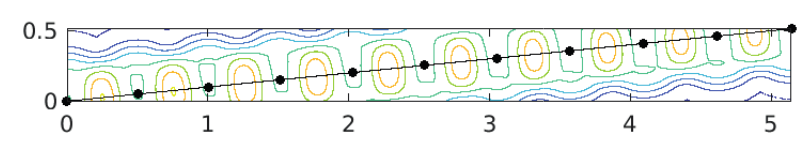
\includegraphics[width=0.5\linewidth]{slow_newton_contour}
	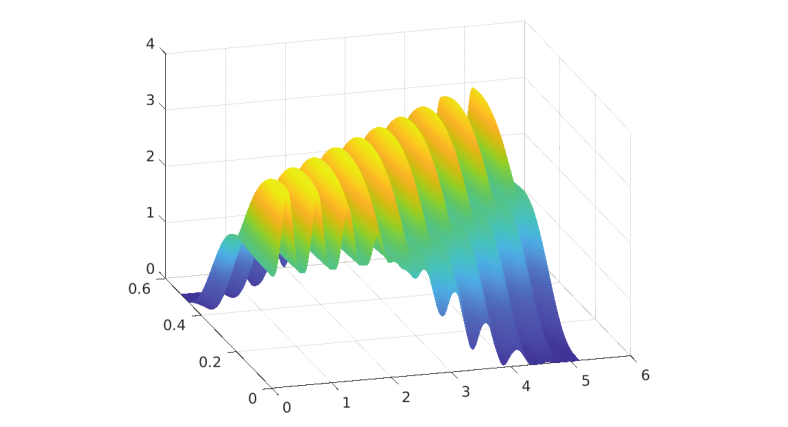
\includegraphics[width=0.5\linewidth]{slow_newton_3d}
	\caption{Contour lines of $f_{SN}(x)$ and the path of iterates for $k = 0, . . . , 10$. Below a 3D view of the function.}
\end{figure}
\noindent Despite all the negative results listed here, Newton's method does have one very attractive feature: one can prove local quadratic rate of convergence, which means that near the optimal solution the errors $e_k = \|x_k - x^*\|$ (where $x^*$ is the unique optimal solution) satisfy the inequality $e_{k+1} \leq M e_k^2$ for some positive $M > 0$. This property essentially means that the number of accuracy digits is doubled at each iteration.

\begin{theorem}[Quadratic local convergence of Newton's method]\label{thm:newton}
	Let $f\in \Cii(\Rn)$ with $\hess$ Lipschitz continuous. Moreover, let $\hess(x)$ be positive definite for any $x \in \mathbb{R}^n$. Let $\{x_k\}_{k \geq 0}$ be the sequence generated by Algorithm \ref{alg:newton}, and let $x^*$ be the unique minimizer of $f$ over $\mathbb{R}^n$. Then, we have 
	\begin{equation}\label{eq:newton_contraction}
		\|x_{k+1} - x^*\| \leq \frac{L}{2m}\|x_k - x^*\|^2 \quad \forall k = 0, 1, \ldots
	\end{equation}
	holds. In addition, if $\|x_0 - x^*\| \leq \frac{m}{L}$, then
	\begin{equation}\label{eq:local_newton}
		\|x_k - x^*\| \leq \frac{2m}{L} \left(\frac{1}{2}\right)^{2^k}.
	\end{equation}
\end{theorem}
\begin{proof}
	Let $k$ be a nonnegative integer. Then, from  $\grad(x^*)=0$ and the fundamental Theorem of Calculus, we have
	\begin{align*}
		x_{k+1} - x^* &= x_k - (\hess(x_k))^{-1} \grad(x_k) - x^* \nonumber \\
		&= x_k - x^* + (\hess(x_k))^{-1}(\grad(x^*) - \grad(x_k)) \nonumber \\
		&= x_k - x^* + (\hess(x_k))^{-1} \int_0^1 [\hess(x_k + t(x^* - x_k))](x^* - x_k) dt \nonumber \\
		&= (\hess(x_k))^{-1} \int_0^1 [\hess(x_k + t(x^* - x_k)) - \hess(x_k)](x^* - x_k) dt. \nonumber
	\end{align*}
	Combining the latter equality with the fact that $\hess(x)\succ 0 \forall x,$ i.e., $\exists m>0: \hess(x_k) \succeq mI$, implies that $\|(\hess(x_k))^{-1}\| \leq \frac{1}{m}$. Hence,
	\begin{align*}
		\|x_{k+1} - x^*\| &\leq \|(\hess(x_k))^{-1}\| \left\| \int_0^1 [\hess(x_k + t(x^* - x_k)) - \hess(x_k)](x^* - x_k) dt \right\| \nonumber \\
		&\leq \|(\hess(x_k))^{-1}\| \int_0^1 \left\| [\hess(x_k + t(x^* - x_k)) - \hess(x_k)](x^* - x_k) \right\| dt \nonumber \\
		&\leq \|(\hess(x_k))^{-1}\| \int_0^1 \|\hess(x_k + t(x^* - x_k)) - \hess(x_k)\| \cdot \|x^* - x_k\| dt \nonumber \\
		&\leq \frac{L}{m} \int_0^1 t \|x_k - x^*\|^2 dt = \frac{L}{2m} \|x_k - x^*\|^2, \nonumber
	\end{align*}
where the last inequality follows from the Lipschitz continuity of the Hessian.	Now, we will prove inequality \eqref{eq:local_newton} by induction on $k$. Note that for $k = 0$, we assumed that
	\begin{equation*}
		\|x_0 - x^*\| \leq \frac{m}{L},
	\end{equation*}	
	so in particular
	\begin{equation*}
		\|x_0 - x^*\| \leq \frac{2m}{L} \left(\frac{1}{2}\right)^{2^0},
	\end{equation*}
	establishing the basis of the induction. Assuming that \eqref{eq:local_newton} holds for an integer $k$, that is, $\|x_k - x^*\| \leq \frac{2m}{L} \left(\frac{1}{2}\right)^{2^k}$, we will show it holds for $k + 1$. Indeed, by \eqref{eq:newton_contraction} we have
	\begin{equation*}
		\|x_{k+1} - x^*\| \leq \frac{L}{2m} \|x_k - x^*\|^2 \leq \frac{L}{2m} \left(\frac{2m}{L} \left(\frac{1}{2}\right)^{2^k}\right)^2 = \frac{2m}{L} \left(\frac{1}{2}\right)^{2^{k+1}},
	\end{equation*}
	proving the desired result.
\end{proof}
\noindent Now, in order to ensure \textbf{global convergence} and maintain this local property, we can employ one of the following globalization techniques:
\begin{itemize}
	\item \textbf{Line search} techniques applied to a descent direction constructed from Newton's direction;
	\item \textbf{Trust region} methods, where $s_k$ is chosen as the optimal solution (with a certain degree of approximation) of
	\begin{equation*}
		\min_{\|s_k\| \leq \Delta_k} q_k(s_k), \quad \with s_k:=x-x_k
	\end{equation*}
	appropriately updating the trust region radius $\Delta_k$ along the iterations (approximations of $\nabla^2 f(x_k)$ can be used);
	\item \textbf{Regularized} methods, where $s_k$ is chosen as the optimal solution (with a certain degree of approximation) of
	\begin{equation*}
		\min_{s_k \in \mathbb{R}^n} q_k(s_k) + \sigma_k \|s_k\|^3
	\end{equation*}
	appropriately updating $\sigma_k$ along the iterations (approximations of $\nabla^2 f(x_k)$ can be used).
\end{itemize}



\section{Truncated Newton with Conjugate Gradient}
The Theorem \ref{thm:newton} above can be relaxed as follows. In particular, we can inexactly solve the Newton equation.
\begin{proposition}[Local Convergence of Inexact Newton]\label{inexact_newton}
	Let $f\in \Cii(\mathcal{D})$ where $\mathcal{D} \subseteq \mathbb{R}^n$ is an open set. Suppose that the following conditions hold:
	\begin{itemize}
		\item[(i)] there exists a point $x^* \in \mathcal{D}$ such that $\nabla f(x^*) = 0$;
		\item[(ii)] the Hessian matrix $\nabla^2 f(x^*)$ is non singular.
	\end{itemize}
	Then, there exist an open ball $\mathcal{B}(x^*; r) \subset \mathcal{D}$, and a value $\bar{\eta}$ such that, if $x_0 \in \mathcal{B}(x^*; r)$ and $\eta_k \in [0, \bar{\eta}]$ for all $k$, then the sequence $\{x_k\}$ generated by the inexact Newton method and defined by the iteration $x_{k+1} = x_k + d_k$, where $d_k$ satisfies the condition
	\begin{equation*}
		\| \nabla q_k(d_k)\|=\|\nabla^2 f(x_k) d_k + \nabla f(x_k)\| \leq \eta_k \|\nabla f(x_k)\|,
	\end{equation*}
	converges to $x^*$ with (at least) linear convergence rate. Moreover 
	\begin{itemize}
		\item[(a)] if $\eta_k \to 0$ then $\{x_k\}$ converges with superlinear convergence rate, i.e., 
		$$ \lim_{k\to \infty} \frac{||x_{k+1}-x^*||}{||x_k-x^*||}=0;$$
		\item[(b)] if the Hessian matrix $\nabla^2 f$ is Lipschitz-continuous on $\mathcal{D}$, and there exists a constant $C > 0$ such that $\eta_k \leq C \|\nabla f(x_k)\|$ for all $k$, then $\{x_k\}$ converges with (at least) quadratic convergence rate.
	\end{itemize}
\end{proposition}
\noindent In case the solution of the Newton equation is constructed via an iterative procedure, the "premature" interruption is called "truncation". In the following algorithm we omit the iteration counter $k$ inside the CG procedure (all the variables there should actually have both the $k$ and $i$ subscripts).\\
\begin{algorithm}[H]\label{alg:tn}
\caption{Truncated Newton with Conjugate Gradient (TNCG)}

\KwIn{Pick $x_0\in \Rn$ arbitrarly, $\eta > 0$, $\epsilon > 0$, $\epsilon_2 > 0$}

$k=0$

\While{$||\grad(x_k)|| > \epsilon$}{
	
	$i = 0$, $d_0 = 0$, $s_0 = -\nabla q_0 = -\nabla f(x_k)$
	
	\While{True}{
		
		\If{$s_i^T \nabla^2 f(x_k) s_i \leq \epsilon_2 \|s_i\|^2$}{		
		
			$d_k = \begin{cases}
				-\nabla f(x_k), & \text{if } i = 0, \\
				d_i, & \text{if } i > 0
			\end{cases}$
	
			\textbf{break}
		}
	
		$\alpha_i = -\frac{\nabla q_i^T s_i}{s_i^T \nabla^2 f(x_k) s_i}$
		
		$d_{i+1} = d_i + \alpha_i s_i$
		
		$\nabla q_{i+1} = \nabla q_i + \alpha_i \nabla^2 f(x_k) s_i.$
		
		\If{$\|\nabla q_i\| \leq \eta \|\nabla f(x_k)\| \min\left\{\frac{1}{k+1}, \|\nabla f(x_k)\|\right\}$}{
			
			$d_k = d_i$
			
			\textbf{break}
		}
	
		$\beta_{i+1} = \frac{\nabla q_{i+1}^T \nabla^2 f(x_k) s_i}{s_i^T \nabla^2 f(x_k) s_i}$
		
		$s_{i+1} = -\nabla q_{i+1} + \beta_{i+1} s_i,$
		
		$i= i+1$
	}
	
	$t_k \leftarrow$ Line Search along $d_k$ with 1 as initial step.
	
	$x_{k+1} = x_k +t_k d_k$
	
	$k = k+1$
}
\end{algorithm}
\noindent Given that $d_{k,0}=-\grad(x_k)$, CG is iteratively refining a gradient direction into a Newton direction (see Proposition \ref{inexact_newton}).
\end{document}